\documentclass[1p]{elsarticle_modified}
%\bibliographystyle{elsarticle-num}

%\usepackage[colorlinks]{hyperref}
%\usepackage{abbrmath_seonhwa} %\Abb, \Ascr, \Acal ,\Abf, \Afrak
\usepackage{amsfonts}
\usepackage{amssymb}
\usepackage{amsmath}
\usepackage{amsthm}
\usepackage{scalefnt}
\usepackage{amsbsy}
\usepackage{kotex}
\usepackage{caption}
\usepackage{subfig}
\usepackage{color}
\usepackage{graphicx}
\usepackage{xcolor} %% white, black, red, green, blue, cyan, magenta, yellow
\usepackage{float}
\usepackage{setspace}
\usepackage{hyperref}

\usepackage{tikz}
\usetikzlibrary{arrows}

\usepackage{multirow}
\usepackage{array} % fixed length table
\usepackage{hhline}

%%%%%%%%%%%%%%%%%%%%%
\makeatletter
\renewcommand*\env@matrix[1][\arraystretch]{%
	\edef\arraystretch{#1}%
	\hskip -\arraycolsep
	\let\@ifnextchar\new@ifnextchar
	\array{*\c@MaxMatrixCols c}}
\makeatother %https://tex.stackexchange.com/questions/14071/how-can-i-increase-the-line-spacing-in-a-matrix
%%%%%%%%%%%%%%%

\usepackage[normalem]{ulem}

\newcommand{\msout}[1]{\ifmmode\text{\sout{\ensuremath{#1}}}\else\sout{#1}\fi}
%SOURCE: \msout is \stkout macro in https://tex.stackexchange.com/questions/20609/strikeout-in-math-mode

\newcommand{\cancel}[1]{
	\ifmmode
	{\color{red}\msout{#1}}
	\else
	{\color{red}\sout{#1}}
	\fi
}

\newcommand{\add}[1]{
	{\color{blue}\uwave{#1}}
}

\newcommand{\replace}[2]{
	\ifmmode
	{\color{red}\msout{#1}}{\color{blue}\uwave{#2}}
	\else
	{\color{red}\sout{#1}}{\color{blue}\uwave{#2}}
	\fi
}

\newcommand{\Sol}{\mathcal{S}} %segment
\newcommand{\D}{D} %diagram
\newcommand{\A}{\mathcal{A}} %arc


%%%%%%%%%%%%%%%%%%%%%%%%%%%%%5 test

\def\sl{\operatorname{\textup{SL}}(2,\Cbb)}
\def\psl{\operatorname{\textup{PSL}}(2,\Cbb)}
\def\quan{\mkern 1mu \triangleright \mkern 1mu}

\theoremstyle{definition}
\newtheorem{thm}{Theorem}[section]
\newtheorem{prop}[thm]{Proposition}
\newtheorem{lem}[thm]{Lemma}
\newtheorem{ques}[thm]{Question}
\newtheorem{cor}[thm]{Corollary}
\newtheorem{defn}[thm]{Definition}
\newtheorem{exam}[thm]{Example}
\newtheorem{rmk}[thm]{Remark}
\newtheorem{alg}[thm]{Algorithm}

\newcommand{\I}{\sqrt{-1}}
\begin{document}

%\begin{frontmatter}
%
%\title{Boundary parabolic representations of knots up to 8 crossings}
%
%%% Group authors per affiliation:
%\author{Yunhi Cho} 
%\address{Department of Mathematics, University of Seoul, Seoul, Korea}
%\ead{yhcho@uos.ac.kr}
%
%
%\author{Seonhwa Kim} %\fnref{s_kim}}
%\address{Center for Geometry and Physics, Institute for Basic Science, Pohang, 37673, Korea}
%\ead{ryeona17@ibs.re.kr}
%
%\author{Hyuk Kim}
%\address{Department of Mathematical Sciences, Seoul National University, Seoul 08826, Korea}
%\ead{hyukkim@snu.ac.kr}
%
%\author{Seokbeom Yoon}
%\address{Department of Mathematical Sciences, Seoul National University, Seoul, 08826,  Korea}
%\ead{sbyoon15@snu.ac.kr}
%
%\begin{abstract}
%We find all boundary parabolic representation of knots up to 8 crossings.
%
%\end{abstract}
%\begin{keyword}
%    \MSC[2010] 57M25 
%\end{keyword}
%
%\end{frontmatter}

%\linenumbers
%\tableofcontents
%
\newcommand\colored[1]{\textcolor{white}{\rule[-0.35ex]{0.8em}{1.4ex}}\kern-0.8em\color{red} #1}%
%\newcommand\colored[1]{\textcolor{white}{ #1}\kern-2.17ex	\textcolor{white}{ #1}\kern-1.81ex	\textcolor{white}{ #1}\kern-2.15ex\color{red}#1	}

{\Large $\underline{12n_{0640}~(K12n_{0640})}$}

\setlength{\tabcolsep}{10pt}
\renewcommand{\arraystretch}{1.6}
\vspace{1cm}\begin{tabular}{m{100pt}>{\centering\arraybackslash}m{274pt}}
\multirow{5}{120pt}{
	\centering
	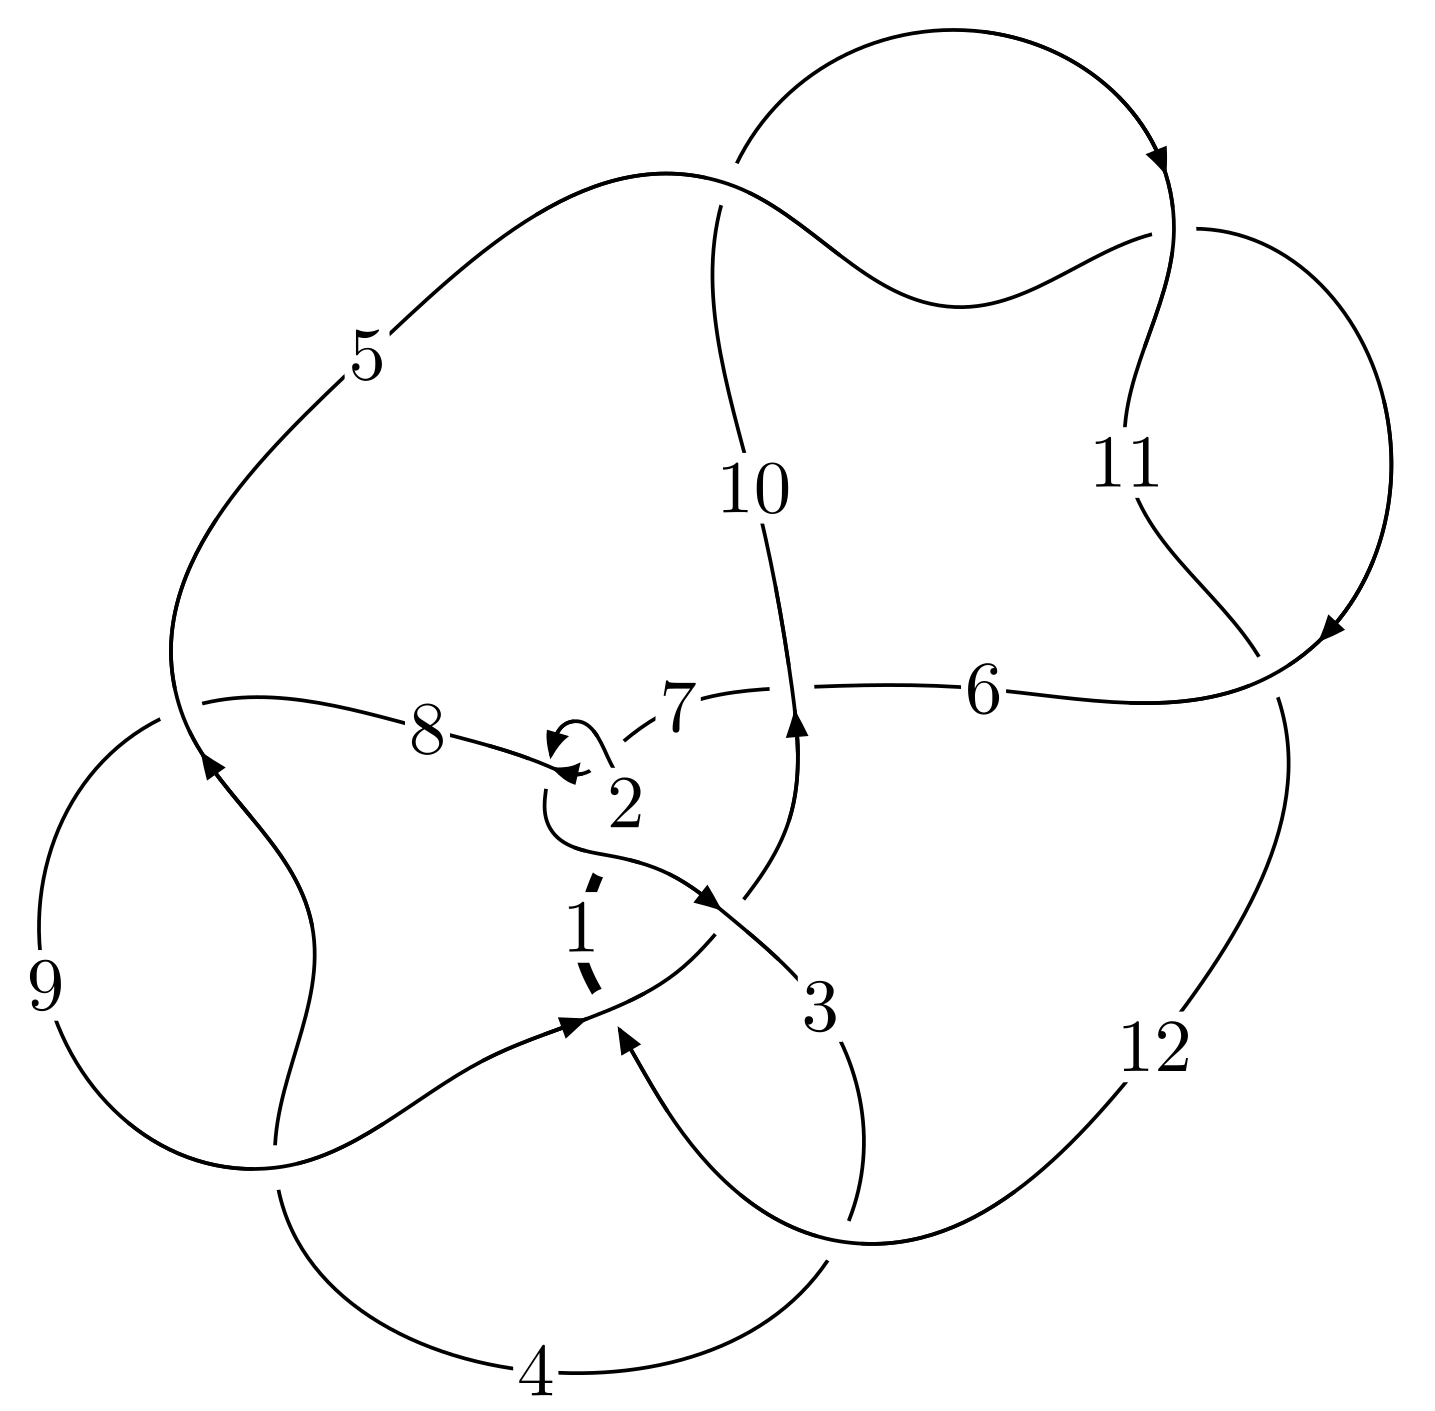
\includegraphics[width=112pt]{../../../GIT/diagram.site/Diagrams/png/2729_12n_0640.png}\\
\ \ \ A knot diagram\footnotemark}&
\allowdisplaybreaks
\textbf{Linearized knot diagam} \\
\cline{2-2}
 &
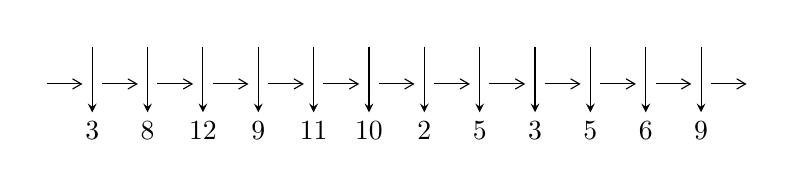
\begin{tikzpicture}[x=20pt, y=17pt]
	% nodes
	\node (C0) at (0, 0) {};
	\node (C1) at (1, 0) {};
	\node (C1U) at (1, +1) {};
	\node (C1D) at (1, -1) {3};

	\node (C2) at (2, 0) {};
	\node (C2U) at (2, +1) {};
	\node (C2D) at (2, -1) {8};

	\node (C3) at (3, 0) {};
	\node (C3U) at (3, +1) {};
	\node (C3D) at (3, -1) {12};

	\node (C4) at (4, 0) {};
	\node (C4U) at (4, +1) {};
	\node (C4D) at (4, -1) {9};

	\node (C5) at (5, 0) {};
	\node (C5U) at (5, +1) {};
	\node (C5D) at (5, -1) {11};

	\node (C6) at (6, 0) {};
	\node (C6U) at (6, +1) {};
	\node (C6D) at (6, -1) {10};

	\node (C7) at (7, 0) {};
	\node (C7U) at (7, +1) {};
	\node (C7D) at (7, -1) {2};

	\node (C8) at (8, 0) {};
	\node (C8U) at (8, +1) {};
	\node (C8D) at (8, -1) {5};

	\node (C9) at (9, 0) {};
	\node (C9U) at (9, +1) {};
	\node (C9D) at (9, -1) {3};

	\node (C10) at (10, 0) {};
	\node (C10U) at (10, +1) {};
	\node (C10D) at (10, -1) {5};

	\node (C11) at (11, 0) {};
	\node (C11U) at (11, +1) {};
	\node (C11D) at (11, -1) {6};

	\node (C12) at (12, 0) {};
	\node (C12U) at (12, +1) {};
	\node (C12D) at (12, -1) {9};
	\node (C13) at (13, 0) {};

	% arrows
	\draw[->,>={angle 60}]
	(C0) edge (C1) (C1) edge (C2) (C2) edge (C3) (C3) edge (C4) (C4) edge (C5) (C5) edge (C6) (C6) edge (C7) (C7) edge (C8) (C8) edge (C9) (C9) edge (C10) (C10) edge (C11) (C11) edge (C12) (C12) edge (C13) ;	\draw[->,>=stealth]
	(C1U) edge (C1D) (C2U) edge (C2D) (C3U) edge (C3D) (C4U) edge (C4D) (C5U) edge (C5D) (C6U) edge (C6D) (C7U) edge (C7D) (C8U) edge (C8D) (C9U) edge (C9D) (C10U) edge (C10D) (C11U) edge (C11D) (C12U) edge (C12D) ;
	\end{tikzpicture} \\
\hhline{~~} \\& 
\textbf{Solving Sequence} \\ \cline{2-2} 
 &
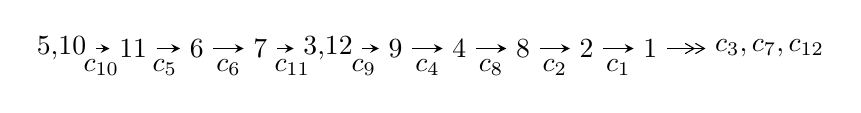
\begin{tikzpicture}[x=23pt, y=7pt]
	% node
	\node (A0) at (-1/8, 0) {5,10};
	\node (A1) at (1, 0) {11};
	\node (A2) at (2, 0) {6};
	\node (A3) at (3, 0) {7};
	\node (A4) at (65/16, 0) {3,12};
	\node (A5) at (41/8, 0) {9};
	\node (A6) at (49/8, 0) {4};
	\node (A7) at (57/8, 0) {8};
	\node (A8) at (65/8, 0) {2};
	\node (A9) at (73/8, 0) {1};
	\node (C1) at (1/2, -1) {$c_{10}$};
	\node (C2) at (3/2, -1) {$c_{5}$};
	\node (C3) at (5/2, -1) {$c_{6}$};
	\node (C4) at (7/2, -1) {$c_{11}$};
	\node (C5) at (37/8, -1) {$c_{9}$};
	\node (C6) at (45/8, -1) {$c_{4}$};
	\node (C7) at (53/8, -1) {$c_{8}$};
	\node (C8) at (61/8, -1) {$c_{2}$};
	\node (C9) at (69/8, -1) {$c_{1}$};
	\node (A10) at (11, 0) {$c_{3},c_{7},c_{12}$};

	% edge
	\draw[->,>=stealth]	
	(A0) edge (A1) (A1) edge (A2) (A2) edge (A3) (A3) edge (A4) (A4) edge (A5) (A5) edge (A6) (A6) edge (A7) (A7) edge (A8) (A8) edge (A9) ;
	\draw[->>,>={angle 60}]	
	(A9) edge (A10);
\end{tikzpicture} \\ 

\end{tabular} \\

\footnotetext{
The image of knot diagram is generated by the software ``\textbf{Draw programme}" developed by Andrew Bartholomew(\url{http://www.layer8.co.uk/maths/draw/index.htm\#Running-draw}), where we modified some parts for our purpose(\url{https://github.com/CATsTAILs/LinksPainter}).
}\phantom \\ \newline 
\centering \textbf{Ideals for irreducible components\footnotemark of $X_{\text{par}}$} 
 
\begin{align*}
I^u_{1}&=\langle 
9.89972\times10^{17} u^{23}-1.91877\times10^{15} u^{22}+\cdots+4.06813\times10^{18} b-2.49679\times10^{18},\\
\phantom{I^u_{1}}&\phantom{= \langle  }8.63753\times10^{17} u^{23}-1.70899\times10^{18} u^{22}+\cdots+4.06813\times10^{18} a-1.68305\times10^{19},\;u^{24}-10 u^{22}+\cdots+6 u+1\rangle \\
I^u_{2}&=\langle 
u^{11}-7 u^9+17 u^7+u^6-15 u^5-3 u^4+2 u^2+b+3 u,\\
\phantom{I^u_{2}}&\phantom{= \langle  }u^9- u^8-6 u^7+6 u^6+11 u^5-11 u^4-5 u^3+6 u^2+a-3 u+1,\\
\phantom{I^u_{2}}&\phantom{= \langle  }u^{12}-8 u^{10}+24 u^8+u^7-32 u^6-4 u^5+15 u^4+5 u^3+2 u^2-2 u-1\rangle \\
I^u_{3}&=\langle 
b,\;a-1,\;u-1\rangle \\
\\
\end{align*}
\raggedright * 3 irreducible components of $\dim_{\mathbb{C}}=0$, with total 37 representations.\\
\footnotetext{All coefficients of polynomials are rational numbers. But the coefficients are sometimes approximated in decimal forms when there is not enough margin.}
\newpage
\renewcommand{\arraystretch}{1}
\centering \section*{I. $I^u_{1}= \langle 9.90\times10^{17} u^{23}-1.92\times10^{15} u^{22}+\cdots+4.07\times10^{18} b-2.50\times10^{18},\;8.64\times10^{17} u^{23}-1.71\times10^{18} u^{22}+\cdots+4.07\times10^{18} a-1.68\times10^{19},\;u^{24}-10 u^{22}+\cdots+6 u+1 \rangle$}
\flushleft \textbf{(i) Arc colorings}\\
\begin{tabular}{m{7pt} m{180pt} m{7pt} m{180pt} }
\flushright $a_{5}=$&$\begin{pmatrix}0\\u\end{pmatrix}$ \\
\flushright $a_{10}=$&$\begin{pmatrix}1\\0\end{pmatrix}$ \\
\flushright $a_{11}=$&$\begin{pmatrix}1\\u^2\end{pmatrix}$ \\
\flushright $a_{6}=$&$\begin{pmatrix}- u\\- u^3+u\end{pmatrix}$ \\
\flushright $a_{7}=$&$\begin{pmatrix}u^3-2 u\\- u^3+u\end{pmatrix}$ \\
\flushright $a_{3}=$&$\begin{pmatrix}-0.212322 u^{23}+0.420093 u^{22}+\cdots+3.09567 u+4.13716\\-0.243348 u^{23}+0.000471658 u^{22}+\cdots+1.81524 u+0.613744\end{pmatrix}$ \\
\flushright $a_{12}=$&$\begin{pmatrix}- u^2+1\\- u^4+2 u^2\end{pmatrix}$ \\
\flushright $a_{9}=$&$\begin{pmatrix}-1.25860 u^{23}+0.336558 u^{22}+\cdots-22.2342 u-4.64549\\-0.0840693 u^{23}+0.188815 u^{22}+\cdots-7.10991 u-1.40341\end{pmatrix}$ \\
\flushright $a_{4}=$&$\begin{pmatrix}-0.483379 u^{23}+0.505798 u^{22}+\cdots-2.99675 u+2.78091\\-0.208694 u^{23}-0.00110386 u^{22}+\cdots+1.55323 u+0.479053\end{pmatrix}$ \\
\flushright $a_{8}=$&$\begin{pmatrix}-1.25860 u^{23}+0.336558 u^{22}+\cdots-22.2342 u-4.64549\\-0.226293 u^{23}+0.0998004 u^{22}+\cdots-6.34916 u-1.06686\end{pmatrix}$ \\
\flushright $a_{2}=$&$\begin{pmatrix}-1.51744 u^{23}+0.547755 u^{22}+\cdots-19.4211 u-3.44143\\-0.320558 u^{23}+0.0501945 u^{22}+\cdots-5.21590 u-0.630497\end{pmatrix}$ \\
\flushright $a_{1}=$&$\begin{pmatrix}1.40524 u^{23}-0.275084 u^{22}+\cdots+14.6942 u+2.32021\\0.344813 u^{23}-0.0300623 u^{22}+\cdots-3.26431 u-0.145094\end{pmatrix}$\\&\end{tabular}
\flushleft \textbf{(ii) Obstruction class $= -1$}\\~\\
\flushleft \textbf{(iii) Cusp Shapes $= -\frac{18808788651478118843}{4068132824722451189} u^{23}+\frac{899618609945270896}{4068132824722451189} u^{22}+\cdots-\frac{136381012325864299426}{4068132824722451189} u-\frac{118763470922061227713}{4068132824722451189}$}\\~\\
\newpage\renewcommand{\arraystretch}{1}
\flushleft \textbf{(iv) u-Polynomials at the component}\newline \\
\begin{tabular}{m{50pt}|m{274pt}}
Crossings & \hspace{64pt}u-Polynomials at each crossing \\
\hline $$\begin{aligned}c_{1}\end{aligned}$$&$\begin{aligned}
&u^{24}+4 u^{23}+\cdots+1789 u+1
\end{aligned}$\\
\hline $$\begin{aligned}c_{2},c_{7}\end{aligned}$$&$\begin{aligned}
&u^{24}+2 u^{23}+\cdots+47 u+1
\end{aligned}$\\
\hline $$\begin{aligned}c_{3}\end{aligned}$$&$\begin{aligned}
&u^{24}-3 u^{23}+\cdots+14 u+1
\end{aligned}$\\
\hline $$\begin{aligned}c_{4},c_{8}\end{aligned}$$&$\begin{aligned}
&u^{24}+3 u^{23}+\cdots+80 u+19
\end{aligned}$\\
\hline $$\begin{aligned}c_{5},c_{10},c_{11}\end{aligned}$$&$\begin{aligned}
&u^{24}-10 u^{22}+\cdots+6 u+1
\end{aligned}$\\
\hline $$\begin{aligned}c_{6}\end{aligned}$$&$\begin{aligned}
&u^{24}+3 u^{23}+\cdots+696 u+37
\end{aligned}$\\
\hline $$\begin{aligned}c_{9}\end{aligned}$$&$\begin{aligned}
&u^{24}- u^{23}+\cdots+40 u-8
\end{aligned}$\\
\hline $$\begin{aligned}c_{12}\end{aligned}$$&$\begin{aligned}
&u^{24}+2 u^{23}+\cdots+5 u-1
\end{aligned}$\\
\hline
\end{tabular}\\~\\
\newpage\renewcommand{\arraystretch}{1}
\flushleft \textbf{(v) Riley Polynomials at the component}\newline \\
\begin{tabular}{m{50pt}|m{274pt}}
Crossings & \hspace{64pt}Riley Polynomials at each crossing \\
\hline $$\begin{aligned}c_{1}\end{aligned}$$&$\begin{aligned}
&y^{24}+44 y^{23}+\cdots-3160089 y+1
\end{aligned}$\\
\hline $$\begin{aligned}c_{2},c_{7}\end{aligned}$$&$\begin{aligned}
&y^{24}-4 y^{23}+\cdots-1789 y+1
\end{aligned}$\\
\hline $$\begin{aligned}c_{3}\end{aligned}$$&$\begin{aligned}
&y^{24}+13 y^{23}+\cdots-214 y+1
\end{aligned}$\\
\hline $$\begin{aligned}c_{4},c_{8}\end{aligned}$$&$\begin{aligned}
&y^{24}+29 y^{23}+\cdots-5754 y+361
\end{aligned}$\\
\hline $$\begin{aligned}c_{5},c_{10},c_{11}\end{aligned}$$&$\begin{aligned}
&y^{24}-20 y^{23}+\cdots-26 y+1
\end{aligned}$\\
\hline $$\begin{aligned}c_{6}\end{aligned}$$&$\begin{aligned}
&y^{24}+47 y^{23}+\cdots-161850 y+1369
\end{aligned}$\\
\hline $$\begin{aligned}c_{9}\end{aligned}$$&$\begin{aligned}
&y^{24}+23 y^{23}+\cdots-4064 y+64
\end{aligned}$\\
\hline $$\begin{aligned}c_{12}\end{aligned}$$&$\begin{aligned}
&y^{24}-60 y^{23}+\cdots-93 y+1
\end{aligned}$\\
\hline
\end{tabular}\\~\\
\newpage\flushleft \textbf{(vi) Complex Volumes and Cusp Shapes}
$$\begin{array}{c|c|c}  
\text{Solutions to }I^u_{1}& \I (\text{vol} + \sqrt{-1}CS) & \text{Cusp shape}\\
 \hline 
\begin{aligned}
u &= \phantom{-}0.797828 + 0.678753 I \\
a &= -1.02319 + 1.10302 I \\
b &= -0.55673 - 1.65487 I\end{aligned}
 & \phantom{-}3.88067 - 2.62654 I & -11.07995 + 2.70331 I \\ \hline\begin{aligned}
u &= \phantom{-}0.797828 - 0.678753 I \\
a &= -1.02319 - 1.10302 I \\
b &= -0.55673 + 1.65487 I\end{aligned}
 & \phantom{-}3.88067 + 2.62654 I & -11.07995 - 2.70331 I \\ \hline\begin{aligned}
u &= \phantom{-}1.05078\phantom{ +0.000000I} \\
a &= \phantom{-}0.906274\phantom{ +0.000000I} \\
b &= \phantom{-}0.133759\phantom{ +0.000000I}\end{aligned}
 & -4.93398\phantom{ +0.000000I} & -18.0800\phantom{ +0.000000I} \\ \hline\begin{aligned}
u &= \phantom{-}1.21774\phantom{ +0.000000I} \\
a &= \phantom{-}1.31377\phantom{ +0.000000I} \\
b &= \phantom{-}1.26448\phantom{ +0.000000I}\end{aligned}
 & -6.34892\phantom{ +0.000000I} & -11.4760\phantom{ +0.000000I} \\ \hline\begin{aligned}
u &= -1.117180 + 0.558107 I \\
a &= \phantom{-}0.264601 + 0.177693 I \\
b &= -0.642330 - 1.001630 I\end{aligned}
 & \phantom{-}0.11807 + 2.01122 I & -11.63298 - 1.47216 I \\ \hline\begin{aligned}
u &= -1.117180 - 0.558107 I \\
a &= \phantom{-}0.264601 - 0.177693 I \\
b &= -0.642330 + 1.001630 I\end{aligned}
 & \phantom{-}0.11807 - 2.01122 I & -11.63298 + 1.47216 I \\ \hline\begin{aligned}
u &= \phantom{-}1.282720 + 0.266061 I \\
a &= -0.417258 + 1.231710 I \\
b &= -0.313111 - 0.558407 I\end{aligned}
 & -2.36903 - 5.36546 I & -17.8756 + 8.3270 I \\ \hline\begin{aligned}
u &= \phantom{-}1.282720 - 0.266061 I \\
a &= -0.417258 - 1.231710 I \\
b &= -0.313111 + 0.558407 I\end{aligned}
 & -2.36903 + 5.36546 I & -17.8756 - 8.3270 I \\ \hline\begin{aligned}
u &= -0.123057 + 1.316600 I \\
a &= \phantom{-}0.002520 - 1.240400 I \\
b &= -0.32423 + 2.21788 I\end{aligned}
 & \phantom{-}10.67480 + 4.86745 I & -9.82219 - 2.45720 I \\ \hline\begin{aligned}
u &= -0.123057 - 1.316600 I \\
a &= \phantom{-}0.002520 + 1.240400 I \\
b &= -0.32423 - 2.21788 I\end{aligned}
 & \phantom{-}10.67480 - 4.86745 I & -9.82219 + 2.45720 I\\
 \hline 
 \end{array}$$\newpage$$\begin{array}{c|c|c}  
\text{Solutions to }I^u_{1}& \I (\text{vol} + \sqrt{-1}CS) & \text{Cusp shape}\\
 \hline 
\begin{aligned}
u &= -1.315130 + 0.199500 I \\
a &= \phantom{-}0.931929 + 0.744429 I \\
b &= \phantom{-}0.399732 - 1.228200 I\end{aligned}
 & -2.04826 + 3.83523 I & -16.1350 - 2.1387 I \\ \hline\begin{aligned}
u &= -1.315130 - 0.199500 I \\
a &= \phantom{-}0.931929 - 0.744429 I \\
b &= \phantom{-}0.399732 + 1.228200 I\end{aligned}
 & -2.04826 - 3.83523 I & -16.1350 + 2.1387 I \\ \hline\begin{aligned}
u &= -0.410599 + 0.509120 I \\
a &= \phantom{-}0.56444 + 1.46880 I \\
b &= \phantom{-}0.821859 + 0.235411 I\end{aligned}
 & \phantom{-}2.03875 + 2.53994 I & -11.82047 - 4.16914 I \\ \hline\begin{aligned}
u &= -0.410599 - 0.509120 I \\
a &= \phantom{-}0.56444 - 1.46880 I \\
b &= \phantom{-}0.821859 - 0.235411 I\end{aligned}
 & \phantom{-}2.03875 - 2.53994 I & -11.82047 + 4.16914 I \\ \hline\begin{aligned}
u &= \phantom{-}1.49784\phantom{ +0.000000I} \\
a &= \phantom{-}0.0823949\phantom{ +0.000000I} \\
b &= -1.05480\phantom{ +0.000000I}\end{aligned}
 & -11.6286\phantom{ +0.000000I} & -23.4910\phantom{ +0.000000I} \\ \hline\begin{aligned}
u &= \phantom{-}0.394751\phantom{ +0.000000I} \\
a &= \phantom{-}1.18127\phantom{ +0.000000I} \\
b &= \phantom{-}1.60965\phantom{ +0.000000I}\end{aligned}
 & -7.19054\phantom{ +0.000000I} & -5.70560\phantom{ +0.000000I} \\ \hline\begin{aligned}
u &= -1.41645 + 0.78202 I \\
a &= -0.817155 - 0.477348 I \\
b &= -0.71160 + 2.00454 I\end{aligned}
 & \phantom{-}6.79929 + 2.45061 I & -11.06872 - 1.28046 I \\ \hline\begin{aligned}
u &= -1.41645 - 0.78202 I \\
a &= -0.817155 + 0.477348 I \\
b &= -0.71160 - 2.00454 I\end{aligned}
 & \phantom{-}6.79929 - 2.45061 I & -11.06872 + 1.28046 I \\ \hline\begin{aligned}
u &= \phantom{-}1.50198 + 0.60802 I \\
a &= \phantom{-}0.868783 - 0.609431 I \\
b &= \phantom{-}1.06909 + 1.77146 I\end{aligned}
 & \phantom{-}5.60719 - 11.65040 I & -12.86830 + 5.47222 I \\ \hline\begin{aligned}
u &= \phantom{-}1.50198 - 0.60802 I \\
a &= \phantom{-}0.868783 + 0.609431 I \\
b &= \phantom{-}1.06909 - 1.77146 I\end{aligned}
 & \phantom{-}5.60719 + 11.65040 I & -12.86830 - 5.47222 I\\
 \hline 
 \end{array}$$\newpage$$\begin{array}{c|c|c}  
\text{Solutions to }I^u_{1}& \I (\text{vol} + \sqrt{-1}CS) & \text{Cusp shape}\\
 \hline 
\begin{aligned}
u &= -0.313467\phantom{ +0.000000I} \\
a &= -0.425309\phantom{ +0.000000I} \\
b &= -0.324845\phantom{ +0.000000I}\end{aligned}
 & -0.515739\phantom{ +0.000000I} & -19.2450\phantom{ +0.000000I} \\ \hline\begin{aligned}
u &= -0.232568 + 0.185578 I \\
a &= \phantom{-}2.34163 + 3.73562 I \\
b &= \phantom{-}0.349022 + 0.617701 I\end{aligned}
 & \phantom{-}2.00166 + 2.59049 I & -13.9321 - 5.9466 I \\ \hline\begin{aligned}
u &= -0.232568 - 0.185578 I \\
a &= \phantom{-}2.34163 - 3.73562 I \\
b &= \phantom{-}0.349022 - 0.617701 I\end{aligned}
 & \phantom{-}2.00166 - 2.59049 I & -13.9321 + 5.9466 I \\ \hline\begin{aligned}
u &= -1.78276\phantom{ +0.000000I} \\
a &= -0.490994\phantom{ +0.000000I} \\
b &= -0.811626\phantom{ +0.000000I}\end{aligned}
 & -16.2087\phantom{ +0.000000I} & -2.53170\phantom{ +0.000000I}\\
 \hline 
 \end{array}$$\newpage\newpage\renewcommand{\arraystretch}{1}
\centering \section*{II. $I^u_{2}= \langle u^{11}-7 u^9+\cdots+b+3 u,\;u^9- u^8+\cdots+a+1,\;u^{12}-8 u^{10}+\cdots-2 u-1 \rangle$}
\flushleft \textbf{(i) Arc colorings}\\
\begin{tabular}{m{7pt} m{180pt} m{7pt} m{180pt} }
\flushright $a_{5}=$&$\begin{pmatrix}0\\u\end{pmatrix}$ \\
\flushright $a_{10}=$&$\begin{pmatrix}1\\0\end{pmatrix}$ \\
\flushright $a_{11}=$&$\begin{pmatrix}1\\u^2\end{pmatrix}$ \\
\flushright $a_{6}=$&$\begin{pmatrix}- u\\- u^3+u\end{pmatrix}$ \\
\flushright $a_{7}=$&$\begin{pmatrix}u^3-2 u\\- u^3+u\end{pmatrix}$ \\
\flushright $a_{3}=$&$\begin{pmatrix}- u^9+u^8+6 u^7-6 u^6-11 u^5+11 u^4+5 u^3-6 u^2+3 u-1\\- u^{11}+7 u^9-17 u^7- u^6+15 u^5+3 u^4-2 u^2-3 u\end{pmatrix}$ \\
\flushright $a_{12}=$&$\begin{pmatrix}- u^2+1\\- u^4+2 u^2\end{pmatrix}$ \\
\flushright $a_{9}=$&$\begin{pmatrix}- u^{11}+u^{10}+\cdots+u+3\\u^{10}-6 u^8+11 u^6+u^5-4 u^4-2 u^3-5 u^2\end{pmatrix}$ \\
\flushright $a_{4}=$&$\begin{pmatrix}u^{11}-8 u^9+u^8+24 u^7-5 u^6-31 u^5+8 u^4+12 u^3-3 u^2+4 u-2\\- u^{11}+7 u^9-17 u^7- u^6+15 u^5+3 u^4-2 u^2-2 u\end{pmatrix}$ \\
\flushright $a_{8}=$&$\begin{pmatrix}- u^{11}+u^{10}+\cdots+u+3\\- u^6+4 u^4-4 u^2- u-1\end{pmatrix}$ \\
\flushright $a_{2}=$&$\begin{pmatrix}- u^9+u^8+6 u^7-6 u^6-11 u^5+11 u^4+5 u^3-5 u^2+3 u-3\\u^{10}-7 u^8+17 u^6+u^5-16 u^4-3 u^3+2 u^2+2 u+2\end{pmatrix}$ \\
\flushright $a_{1}=$&$\begin{pmatrix}u^{11}-8 u^9+u^8+24 u^7-5 u^6-32 u^5+8 u^4+16 u^3-3 u^2-3\\u^{11}+2 u^{10}+\cdots+7 u+3\end{pmatrix}$\\&\end{tabular}
\flushleft \textbf{(ii) Obstruction class $= 1$}\\~\\
\flushleft \textbf{(iii) Cusp Shapes $= -6 u^{11}+4 u^{10}+43 u^9-25 u^8-108 u^7+42 u^6+108 u^5+u^4-21 u^3-40 u^2-14 u-8$}\\~\\
\newpage\renewcommand{\arraystretch}{1}
\flushleft \textbf{(iv) u-Polynomials at the component}\newline \\
\begin{tabular}{m{50pt}|m{274pt}}
Crossings & \hspace{64pt}u-Polynomials at each crossing \\
\hline $$\begin{aligned}c_{1}\end{aligned}$$&$\begin{aligned}
&u^{12}-12 u^{11}+\cdots-15 u+1
\end{aligned}$\\
\hline $$\begin{aligned}c_{2}\end{aligned}$$&$\begin{aligned}
&u^{12}-6 u^{10}+u^9+15 u^8-3 u^7-21 u^6+4 u^5+17 u^4-4 u^3-7 u^2+u+1
\end{aligned}$\\
\hline $$\begin{aligned}c_{3}\end{aligned}$$&$\begin{aligned}
&u^{12}+3 u^{11}+u^{10}-5 u^9-8 u^8-5 u^7+2 u^6+5 u^5+5 u^4+3 u^3-1
\end{aligned}$\\
\hline $$\begin{aligned}c_{4}\end{aligned}$$&$\begin{aligned}
&u^{12}+u^{11}- u^{10}-3 u^8-2 u^7- u^6+u^5+3 u^4+u^3+2 u^2-1
\end{aligned}$\\
\hline $$\begin{aligned}c_{5}\end{aligned}$$&$\begin{aligned}
&u^{12}-8 u^{10}+24 u^8- u^7-32 u^6+4 u^5+15 u^4-5 u^3+2 u^2+2 u-1
\end{aligned}$\\
\hline $$\begin{aligned}c_{6}\end{aligned}$$&$\begin{aligned}
&u^{12}-8 u^{10}+\cdots+2 u-1
\end{aligned}$\\
\hline $$\begin{aligned}c_{7}\end{aligned}$$&$\begin{aligned}
&u^{12}-6 u^{10}- u^9+15 u^8+3 u^7-21 u^6-4 u^5+17 u^4+4 u^3-7 u^2- u+1
\end{aligned}$\\
\hline $$\begin{aligned}c_{8}\end{aligned}$$&$\begin{aligned}
&u^{12}- u^{11}- u^{10}-3 u^8+2 u^7- u^6- u^5+3 u^4- u^3+2 u^2-1
\end{aligned}$\\
\hline $$\begin{aligned}c_{9}\end{aligned}$$&$\begin{aligned}
&u^{12}-2 u^{10}- u^9-3 u^8- u^7+u^6+2 u^5+3 u^4+u^2- u-1
\end{aligned}$\\
\hline $$\begin{aligned}c_{10},c_{11}\end{aligned}$$&$\begin{aligned}
&u^{12}-8 u^{10}+24 u^8+u^7-32 u^6-4 u^5+15 u^4+5 u^3+2 u^2-2 u-1
\end{aligned}$\\
\hline $$\begin{aligned}c_{12}\end{aligned}$$&$\begin{aligned}
&u^{12}-4 u^{11}+\cdots+7 u+1
\end{aligned}$\\
\hline
\end{tabular}\\~\\
\newpage\renewcommand{\arraystretch}{1}
\flushleft \textbf{(v) Riley Polynomials at the component}\newline \\
\begin{tabular}{m{50pt}|m{274pt}}
Crossings & \hspace{64pt}Riley Polynomials at each crossing \\
\hline $$\begin{aligned}c_{1}\end{aligned}$$&$\begin{aligned}
&y^{12}-12 y^{11}+\cdots-43 y+1
\end{aligned}$\\
\hline $$\begin{aligned}c_{2},c_{7}\end{aligned}$$&$\begin{aligned}
&y^{12}-12 y^{11}+\cdots-15 y+1
\end{aligned}$\\
\hline $$\begin{aligned}c_{3}\end{aligned}$$&$\begin{aligned}
&y^{12}-7 y^{11}+\cdots-10 y^2+1
\end{aligned}$\\
\hline $$\begin{aligned}c_{4},c_{8}\end{aligned}$$&$\begin{aligned}
&y^{12}-3 y^{11}+\cdots-4 y+1
\end{aligned}$\\
\hline $$\begin{aligned}c_{5},c_{10},c_{11}\end{aligned}$$&$\begin{aligned}
&y^{12}-16 y^{11}+\cdots-8 y+1
\end{aligned}$\\
\hline $$\begin{aligned}c_{6}\end{aligned}$$&$\begin{aligned}
&y^{12}-16 y^{11}+\cdots-20 y+1
\end{aligned}$\\
\hline $$\begin{aligned}c_{9}\end{aligned}$$&$\begin{aligned}
&y^{12}-4 y^{11}+\cdots-3 y+1
\end{aligned}$\\
\hline $$\begin{aligned}c_{12}\end{aligned}$$&$\begin{aligned}
&y^{12}-24 y^{11}+\cdots+17 y+1
\end{aligned}$\\
\hline
\end{tabular}\\~\\
\newpage\flushleft \textbf{(vi) Complex Volumes and Cusp Shapes}
$$\begin{array}{c|c|c}  
\text{Solutions to }I^u_{2}& \I (\text{vol} + \sqrt{-1}CS) & \text{Cusp shape}\\
 \hline 
\begin{aligned}
u &= \phantom{-}1.17998\phantom{ +0.000000I} \\
a &= \phantom{-}0.800947\phantom{ +0.000000I} \\
b &= \phantom{-}1.82750\phantom{ +0.000000I}\end{aligned}
 & -9.65747\phantom{ +0.000000I} & -15.7210\phantom{ +0.000000I} \\ \hline\begin{aligned}
u &= -1.23606\phantom{ +0.000000I} \\
a &= -1.56622\phantom{ +0.000000I} \\
b &= -1.10566\phantom{ +0.000000I}\end{aligned}
 & -6.93408\phantom{ +0.000000I} & -26.3380\phantom{ +0.000000I} \\ \hline\begin{aligned}
u &= -1.324120 + 0.237549 I \\
a &= \phantom{-}0.849347 + 0.965329 I \\
b &= \phantom{-}0.107633 - 0.994842 I\end{aligned}
 & -1.41781 + 4.88882 I & -10.78753 - 6.22489 I \\ \hline\begin{aligned}
u &= -1.324120 - 0.237549 I \\
a &= \phantom{-}0.849347 - 0.965329 I \\
b &= \phantom{-}0.107633 + 0.994842 I\end{aligned}
 & -1.41781 - 4.88882 I & -10.78753 + 6.22489 I \\ \hline\begin{aligned}
u &= \phantom{-}0.579754\phantom{ +0.000000I} \\
a &= \phantom{-}0.128754\phantom{ +0.000000I} \\
b &= -1.45303\phantom{ +0.000000I}\end{aligned}
 & -7.57612\phantom{ +0.000000I} & -27.2480\phantom{ +0.000000I} \\ \hline\begin{aligned}
u &= -0.136756 + 0.512426 I \\
a &= \phantom{-}1.53089 + 2.63864 I \\
b &= \phantom{-}0.199486 - 0.931452 I\end{aligned}
 & \phantom{-}2.56609 - 2.20336 I & -4.12994 + 0.41603 I \\ \hline\begin{aligned}
u &= -0.136756 - 0.512426 I \\
a &= \phantom{-}1.53089 - 2.63864 I \\
b &= \phantom{-}0.199486 + 0.931452 I\end{aligned}
 & \phantom{-}2.56609 + 2.20336 I & -4.12994 - 0.41603 I \\ \hline\begin{aligned}
u &= \phantom{-}1.46831 + 0.31043 I \\
a &= -0.963926 + 0.306069 I \\
b &= -0.527150 - 0.827184 I\end{aligned}
 & -2.88723 - 0.94663 I & -11.62610 + 0.41133 I \\ \hline\begin{aligned}
u &= \phantom{-}1.46831 - 0.31043 I \\
a &= -0.963926 - 0.306069 I \\
b &= -0.527150 + 0.827184 I\end{aligned}
 & -2.88723 + 0.94663 I & -11.62610 - 0.41133 I \\ \hline\begin{aligned}
u &= \phantom{-}1.58481\phantom{ +0.000000I} \\
a &= \phantom{-}0.328758\phantom{ +0.000000I} \\
b &= -0.536398\phantom{ +0.000000I}\end{aligned}
 & -11.0733\phantom{ +0.000000I} & -8.22380\phantom{ +0.000000I}\\
 \hline 
 \end{array}$$\newpage$$\begin{array}{c|c|c}  
\text{Solutions to }I^u_{2}& \I (\text{vol} + \sqrt{-1}CS) & \text{Cusp shape}\\
 \hline 
\begin{aligned}
u &= -0.371528\phantom{ +0.000000I} \\
a &= -2.93289\phantom{ +0.000000I} \\
b &= \phantom{-}0.802551\phantom{ +0.000000I}\end{aligned}
 & -4.02071\phantom{ +0.000000I} & -7.78700\phantom{ +0.000000I} \\ \hline\begin{aligned}
u &= -1.75183\phantom{ +0.000000I} \\
a &= \phantom{-}0.408041\phantom{ +0.000000I} \\
b &= \phantom{-}0.905098\phantom{ +0.000000I}\end{aligned}
 & -16.4780\phantom{ +0.000000I} & -32.5950\phantom{ +0.000000I}\\
 \hline 
 \end{array}$$\newpage\newpage\renewcommand{\arraystretch}{1}
\centering \section*{III. $I^u_{3}= \langle b,\;a-1,\;u-1 \rangle$}
\flushleft \textbf{(i) Arc colorings}\\
\begin{tabular}{m{7pt} m{180pt} m{7pt} m{180pt} }
\flushright $a_{5}=$&$\begin{pmatrix}0\\1\end{pmatrix}$ \\
\flushright $a_{10}=$&$\begin{pmatrix}1\\0\end{pmatrix}$ \\
\flushright $a_{11}=$&$\begin{pmatrix}1\\1\end{pmatrix}$ \\
\flushright $a_{6}=$&$\begin{pmatrix}-1\\0\end{pmatrix}$ \\
\flushright $a_{7}=$&$\begin{pmatrix}-1\\0\end{pmatrix}$ \\
\flushright $a_{3}=$&$\begin{pmatrix}1\\0\end{pmatrix}$ \\
\flushright $a_{12}=$&$\begin{pmatrix}0\\1\end{pmatrix}$ \\
\flushright $a_{9}=$&$\begin{pmatrix}1\\0\end{pmatrix}$ \\
\flushright $a_{4}=$&$\begin{pmatrix}1\\1\end{pmatrix}$ \\
\flushright $a_{8}=$&$\begin{pmatrix}1\\-1\end{pmatrix}$ \\
\flushright $a_{2}=$&$\begin{pmatrix}2\\-1\end{pmatrix}$ \\
\flushright $a_{1}=$&$\begin{pmatrix}1\\-1\end{pmatrix}$\\&\end{tabular}
\flushleft \textbf{(ii) Obstruction class $= -1$}\\~\\
\flushleft \textbf{(iii) Cusp Shapes $= -18$}\\~\\
\newpage\renewcommand{\arraystretch}{1}
\flushleft \textbf{(iv) u-Polynomials at the component}\newline \\
\begin{tabular}{m{50pt}|m{274pt}}
Crossings & \hspace{64pt}u-Polynomials at each crossing \\
\hline $$\begin{aligned}c_{1},c_{3},c_{12}\end{aligned}$$&$\begin{aligned}
&u+1
\end{aligned}$\\
\hline $$\begin{aligned}c_{2},c_{4},c_{5}\\c_{7},c_{8},c_{10}\\c_{11}\end{aligned}$$&$\begin{aligned}
&u-1
\end{aligned}$\\
\hline $$\begin{aligned}c_{6},c_{9}\end{aligned}$$&$\begin{aligned}
&u
\end{aligned}$\\
\hline
\end{tabular}\\~\\
\newpage\renewcommand{\arraystretch}{1}
\flushleft \textbf{(v) Riley Polynomials at the component}\newline \\
\begin{tabular}{m{50pt}|m{274pt}}
Crossings & \hspace{64pt}Riley Polynomials at each crossing \\
\hline $$\begin{aligned}c_{1},c_{2},c_{3}\\c_{4},c_{5},c_{7}\\c_{8},c_{10},c_{11}\\c_{12}\end{aligned}$$&$\begin{aligned}
&y-1
\end{aligned}$\\
\hline $$\begin{aligned}c_{6},c_{9}\end{aligned}$$&$\begin{aligned}
&y
\end{aligned}$\\
\hline
\end{tabular}\\~\\
\newpage\flushleft \textbf{(vi) Complex Volumes and Cusp Shapes}
$$\begin{array}{c|c|c}  
\text{Solutions to }I^u_{3}& \I (\text{vol} + \sqrt{-1}CS) & \text{Cusp shape}\\
 \hline 
\begin{aligned}
u &= \phantom{-}1.00000\phantom{ +0.000000I} \\
a &= \phantom{-}1.00000\phantom{ +0.000000I} \\
b &= \phantom{-0.000000 } 0\end{aligned}
 & -4.93480\phantom{ +0.000000I} & -18.0000\phantom{ +0.000000I}\\
 \hline 
 \end{array}$$\newpage
\newpage\renewcommand{\arraystretch}{1}
\centering \section*{ IV. u-Polynomials}
\begin{tabular}{m{50pt}|m{274pt}}
Crossings & \hspace{64pt}u-Polynomials at each crossing \\
\hline $$\begin{aligned}c_{1}\end{aligned}$$&$\begin{aligned}
&(u+1)(u^{12}-12 u^{11}+\cdots-15 u+1)(u^{24}+4 u^{23}+\cdots+1789 u+1)
\end{aligned}$\\
\hline $$\begin{aligned}c_{2}\end{aligned}$$&$\begin{aligned}
&(u-1)\\
&\cdot(u^{12}-6 u^{10}+u^9+15 u^8-3 u^7-21 u^6+4 u^5+17 u^4-4 u^3-7 u^2+u+1)\\
&\cdot(u^{24}+2 u^{23}+\cdots+47 u+1)
\end{aligned}$\\
\hline $$\begin{aligned}c_{3}\end{aligned}$$&$\begin{aligned}
&(u+1)(u^{12}+3 u^{11}+\cdots+3 u^3-1)\\
&\cdot(u^{24}-3 u^{23}+\cdots+14 u+1)
\end{aligned}$\\
\hline $$\begin{aligned}c_{4}\end{aligned}$$&$\begin{aligned}
&(u-1)(u^{12}+u^{11}- u^{10}-3 u^8-2 u^7- u^6+u^5+3 u^4+u^3+2 u^2-1)\\
&\cdot(u^{24}+3 u^{23}+\cdots+80 u+19)
\end{aligned}$\\
\hline $$\begin{aligned}c_{5}\end{aligned}$$&$\begin{aligned}
&(u-1)(u^{12}-8 u^{10}+\cdots+2 u-1)\\
&\cdot(u^{24}-10 u^{22}+\cdots+6 u+1)
\end{aligned}$\\
\hline $$\begin{aligned}c_{6}\end{aligned}$$&$\begin{aligned}
&u(u^{12}-8 u^{10}+\cdots+2 u-1)(u^{24}+3 u^{23}+\cdots+696 u+37)
\end{aligned}$\\
\hline $$\begin{aligned}c_{7}\end{aligned}$$&$\begin{aligned}
&(u-1)\\
&\cdot(u^{12}-6 u^{10}- u^9+15 u^8+3 u^7-21 u^6-4 u^5+17 u^4+4 u^3-7 u^2- u+1)\\
&\cdot(u^{24}+2 u^{23}+\cdots+47 u+1)
\end{aligned}$\\
\hline $$\begin{aligned}c_{8}\end{aligned}$$&$\begin{aligned}
&(u-1)(u^{12}- u^{11}- u^{10}-3 u^8+2 u^7- u^6- u^5+3 u^4- u^3+2 u^2-1)\\
&\cdot(u^{24}+3 u^{23}+\cdots+80 u+19)
\end{aligned}$\\
\hline $$\begin{aligned}c_{9}\end{aligned}$$&$\begin{aligned}
&u(u^{12}-2 u^{10}- u^9-3 u^8- u^7+u^6+2 u^5+3 u^4+u^2- u-1)\\
&\cdot(u^{24}- u^{23}+\cdots+40 u-8)
\end{aligned}$\\
\hline $$\begin{aligned}c_{10},c_{11}\end{aligned}$$&$\begin{aligned}
&(u-1)(u^{12}-8 u^{10}+\cdots-2 u-1)\\
&\cdot(u^{24}-10 u^{22}+\cdots+6 u+1)
\end{aligned}$\\
\hline $$\begin{aligned}c_{12}\end{aligned}$$&$\begin{aligned}
&(u+1)(u^{12}-4 u^{11}+\cdots+7 u+1)(u^{24}+2 u^{23}+\cdots+5 u-1)
\end{aligned}$\\
\hline
\end{tabular}\newpage\renewcommand{\arraystretch}{1}
\centering \section*{ V. Riley Polynomials}
\begin{tabular}{m{50pt}|m{274pt}}
Crossings & \hspace{64pt}Riley Polynomials at each crossing \\
\hline $$\begin{aligned}c_{1}\end{aligned}$$&$\begin{aligned}
&(y-1)(y^{12}-12 y^{11}+\cdots-43 y+1)(y^{24}+44 y^{23}+\cdots-3160089 y+1)
\end{aligned}$\\
\hline $$\begin{aligned}c_{2},c_{7}\end{aligned}$$&$\begin{aligned}
&(y-1)(y^{12}-12 y^{11}+\cdots-15 y+1)(y^{24}-4 y^{23}+\cdots-1789 y+1)
\end{aligned}$\\
\hline $$\begin{aligned}c_{3}\end{aligned}$$&$\begin{aligned}
&(y-1)(y^{12}-7 y^{11}+\cdots-10 y^2+1)(y^{24}+13 y^{23}+\cdots-214 y+1)
\end{aligned}$\\
\hline $$\begin{aligned}c_{4},c_{8}\end{aligned}$$&$\begin{aligned}
&(y-1)(y^{12}-3 y^{11}+\cdots-4 y+1)(y^{24}+29 y^{23}+\cdots-5754 y+361)
\end{aligned}$\\
\hline $$\begin{aligned}c_{5},c_{10},c_{11}\end{aligned}$$&$\begin{aligned}
&(y-1)(y^{12}-16 y^{11}+\cdots-8 y+1)(y^{24}-20 y^{23}+\cdots-26 y+1)
\end{aligned}$\\
\hline $$\begin{aligned}c_{6}\end{aligned}$$&$\begin{aligned}
&y(y^{12}-16 y^{11}+\cdots-20 y+1)(y^{24}+47 y^{23}+\cdots-161850 y+1369)
\end{aligned}$\\
\hline $$\begin{aligned}c_{9}\end{aligned}$$&$\begin{aligned}
&y(y^{12}-4 y^{11}+\cdots-3 y+1)(y^{24}+23 y^{23}+\cdots-4064 y+64)
\end{aligned}$\\
\hline $$\begin{aligned}c_{12}\end{aligned}$$&$\begin{aligned}
&(y-1)(y^{12}-24 y^{11}+\cdots+17 y+1)(y^{24}-60 y^{23}+\cdots-93 y+1)
\end{aligned}$\\
\hline
\end{tabular}
\vskip 2pc
\end{document}